\chapter{基于演化算法的半监督序回归技术}
\label{chap:essor}
根据前面对序回归问题的介绍可知,序回归问题中的无标签数据相比较于传统的分类问题缺失了更多的信息,所以如何利用这些无标签数据的挑战更大。上一章介绍了我们提出的基于加权核判别分析的半监督序回归技术(WKFDOR),它通过计算无标签数据的隶属度和加权策略来利用无标签数据,从而更准确地估计类分布。因为WKFDOR算法中使用的权重是否准确将会对学习性能产生重要的影响,所以这一章节中我们将对\autoref{alg_mem}得到的权重进行优化,从而改进WKFDOR算法的性能。优化权重主要通过结合序信息来更准确地估计权重。一方面,这样能够更充分地使用序回归问题的数据信息;另一方面,引入序信息能够更准确地估计权重,最终提升学习性能。
%序回归问题中,同时引入无标签数据和序信息往往使得问题非凸不可导
%To further improve the overall performance, an evolutionary algorithm (i.e., differential evolution) is employed to evolve the weights.

然而,当权重作为\autoref{wkfdor}中的优化变量时,该优化问题是一个非凸且不可导的问题。在\autoref{chap:review}中,我们分析了演化算法在处理这类问题中的优势。所以,我们使用演化算法来改善权重,提出了一种基于演化算法的半监督序回归技术。

在本章中,我们将首先提出基于演化算法的半监督核判别分析序回归算法(Evolutionary Semi-Supervised Ordinal Regression Using Weighted Kernel Fisher Discriminant Analysis,ESSOR)。其次,我们将通过实验来验证演化算法在进一步提升学习性能上的有效性。本章还将介绍在处理大规模数据集上的加速方法。

%然而,当权重作为\autoref{wkfdor}中的优化变量时,该优化问题是一个非凸且不可导的问题。传统的优化算法(例如梯度下降算法)难以处理这种类型的问题,而演化算法(evolutionary algorithm, EA)适用于处理。所以,在这一章中我们使用了演化算法来改善权重,具体的说是差分进化(differential evolution, DE)算法[R. Storn and K. Price, “Differential evolution–a simple and effi- cient heuristic for global optimization over continuous spaces,” Journal of Global Optimization, vol. 11, no. 4, pp. 341–359, 1997.]。差分进化算法是一种高效的处理连续优化问题的演化算法,它简单易用,并且容易并行化。此外,差分进化算法具有收敛好和实现快的属性[K. Price, R. M. Storn, and J. A. Lampinen, Differential Evolu- tion: A Practical Approach to Global Optimization. Secaucus, NJ, USA: Springer-Verlag New York, Inc., 2005.]。因此,我们采用差分进化算法。下面我们首先介绍个体表示(individual representation)方法,即如何表示我们需要优化的变量;其次我们介绍适应度评估函数(fitness function),最后介绍我们提出的基于演化算法的半监督核判别分析序回归算法(evolutionary semi-supervised ordinal regression using weighted kernel Fisher discriminant analysis, ESSOR)。

% \section{演化算法及演化机器学习}
% 在人工智能领域,演化算法(EA)是演化计算的一个子集,是一类基于种群的元启发式优化算法。用种群中的个体来表示优化问题中的候选解,而适应度函数(fitness function)用于决定个体的质量。EA使用类似于生物进化的机制,例如交叉、变异、选择等来实现种群的进化,最终得到满足一定条件的优化问题的解。\autoref{alg_EA}给出了演化算法的基本框架。其中,终止条件一般是代数达到预设的最大代数,或者是计算时间达到限制,或者是适应度达到一定的标准。

% \IncMargin{1em}
% \begin{algorithm}
% \SetKwData{Left}{left}\SetKwData{This}{this}\SetKwData{Up}{up}
% \SetKwFunction{Union}{Union}\SetKwFunction{FindCompress}{FindCompress}
% \SetKwInOut{Input}{input}\SetKwInOut{Output}{output}
% \emph{初始化种群$P(0) = \{x_{1},x_{2},\dots ,x_{N_{p}}\}$}\;
% \emph{令代数计数器$g = 0$}\;
% \emph{评估$P(0)$中每个个体的适应度}\;
% \Repeat{满足EA的终止条件}{
%     \emph{通过交叉、变异、选择等算子,由$P(g)$生成新的种群$P(g+1)$}\;
%     \emph{评估$P(g)$中每个个体的适应度}\;
%     \emph{$g=g+1$}\;
% }
% \caption{演化算法的基本框架}\label{alg_EA}
% \end{algorithm}\DecMargin{1em}

% 优化算法通常可以分为三类:解析法(calculus-based)、枚举法(enumerative)和随机法\citep{潘正君1998演化计算}。解析法在求解过程中需要使用目标函数的解析性质,例如一阶导数、二阶导数等。通常,解析法根据目标函数的梯度信息来确定下一步的搜索方向,如Newton法、共轭梯度下降法等。此外,解析法在求解非凸问题时,往往会根据最陡的方向找到一个局部最优点,而难以找到一个全局最优解。枚举法是一种暴力搜索的方法,它不使用启发信息,而直接对候选的解空间进行逐一枚举计算。对于大规模的优化问题,枚举法速度慢,难以适用。演化算法属于随机法的一种,它使用随机性的转移规则而不是确定性的转移规则,因而能跳出局部最优,搜索到全局较优的解。相比较于解析法,演化算法不需要目标的解析性质,因此它能够处理目标函数不可导的优化问题。此外,相比较于枚举法,演化算法是一种元启发式算法,它能够通过适应度函数和进化算子引导种群的进化,以较快地速度找到全局较优的解。

% EA在求解各种优化问题时,通常都能得到不错的近似解,因为它没有对潜在的适应度曲面做任何假设。尤其是在求解一些非凸、目标函数不可导、甚至连优化目标都难以形式化定义的优化问题时,演化算法具有明显的优势。

%可以把这一小节放到上面去。
%In this circumstance, evolutionary algorithms (EA) are ac- claimed, since they perform well for this type of problems. Recently, EA have been used in many machine learning problems, such as feature extraction [13], pattern recognition [14] and ensemble learning [15].

\section{基于演化算法的半监督核判别分析序回归算法}
%当权重作为\autoref{wkfdor}中的优化变量时,该优化问题是一个非凸且不可导的问题。传统的优化算法(例如梯度下降算法)难以处理这种类型的问题,而演化算法(evolutionary algorithm, EA)适用于处理。
根据前面的分析可知,我们需要借助演化算法来优化权重,进而提升WKFDOR算法的性能。本节我们基于WKFDOR提出改进的算法——ESSOR。下面我们首先介绍个体表示方法,即如何表示我们需要优化的变量;其次介绍适应度评估函数;最后根据问题特点,我们选择了一种处理连续优化问题的演化算法——差分进化算法(Differential Evolution,DE),并给出了ESSOR的算法步骤。

\subsection{个体表示}
最简单直接的方法就是将整个无标签数据的权重矩阵作为一个个体,但是这样的话每个个体的维度将是\((N-L)\times K\)(注意,有标签数据的权重是固定的,我们只需要去优化无标签数据的权重),即和无标签数据量成正比。可以想象,当我们使用大量的无标签数据时,每个个体的维度将非常高,这对演化算法来说无疑是个灾难。因此,我们提出了一个新颖的个体表示方法,它能够将个体大小减小到\(K\)(即序的个数)。

个体的作用是用来表示解空间,使得优化算法能够不断地在适应度函数的引导下在解空间产生更优的个体。在该问题中,我们需要不断更新权重,而新的权重可以用已有的权重通过一定的规则产生。因此,我们考虑将更新权重规则参数化,通过控制这些参数来间接引导权重的更新。我们给第\(k\)个类别引入一个参数\(\lambda_{k}\),并将个体定义为\(\lambda=(\lambda_{1},\lambda_{2},\dots,\lambda_{K})\)。新的权重通过下面的更新规则产生:
\begin{equation}
\label{mem_updateRule}
u_{jk}^{'}=\frac{u_{jk}^{\lambda_{k}}}{\Sigma_{k=1}^{K} u_{jk}^{\lambda_{k}}}
\end{equation}
其中 \(u_{jk}\)是\autoref{alg_mem}估计的权重,将其作为初始权重。新的 \(\mathcal{M}_{k}\) 和 \(\mathcal{N}\)可以通过\autoref{M}和\autoref{N}计算得到,新的投影向量\(w\) 可以通过求解\autoref{wkfdor}的优化问题得到。根据上面的分析,\(\lambda\)引导了无标签数据权重的更新,从而将原问题转化成了搜索最优的\(\lambda\)。注意,有标签数据的权重(即直接从它们的标签可获得)在演化过程中固定不变。

我们对权重更新规则\autoref{mem_updateRule}进行了一定的数学分析,下面的这些特性保证了它能够合理地调整权重:
\begin{enumerate}
\item[1.]对每一个数据点,权重更新规则能够改变它属于两个不同类别的权重的相对值。
\\ \[ \frac{u_{jk_{1}}^{'}}{u_{jk_{2}}^{'}}=\frac{u_{jk_{1}}^{\lambda_{k_{1}}}}{u_{jk_{2}}^{\lambda_{k_{2}}}} \neq \frac{u_{jk_{1}}}{u_{jk_{2}}} \]
%
\item[2.]对两个不同的数据点,权重更新规则能够改变它们属于同一个类别的权重的相对值。
\\ \[ \frac{u_{ik}^{'}}{u_{jk}^{'}}=\frac{u_{ik}^{\lambda_{k}} \sum_{k=1}^{K}u_{jk}^{\lambda_{k}}}{u_{jk}^{\lambda_{k}} \sum_{k=1}^{K}u_{ik}^{\lambda_{k}}} \neq \frac{u_{ik}}{u_{jk}} \]
%
\item[3.]权重的改变不仅和\(\lambda\)相关,同时也受到初始权重的影响。
\\ \[ \frac{u_{ik}^{'}}{u_{ik}}=\frac{u_{ik}^{\lambda_{k}-1}}{\Sigma_{k=1}^{K} u_{ik}^{\lambda_{k}}} \]
\end{enumerate}
为了进一步观察权重更新规则的特性,假设\(\lambda_{k}\)随机取值于一个\([0,2]\)范围内的均匀分布,\autoref{fig_expFunc}画出了一组以不同\(u\)值为底数的指数函数。
\begin{figure}[h]
   \centering
   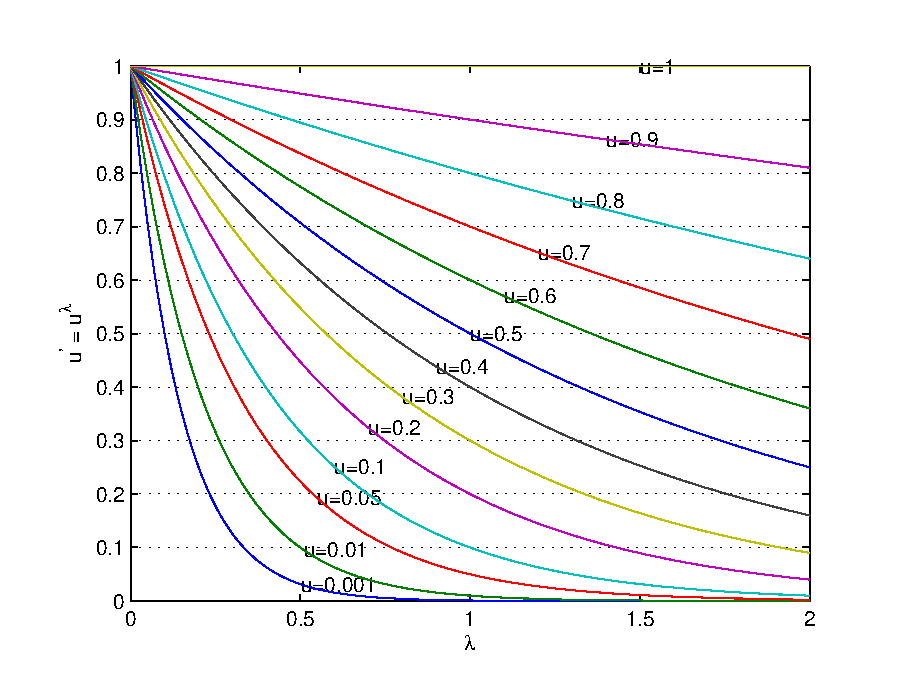
\includegraphics[width=4.5in]{figures/expfunc}
\caption{以不同\(u\)值为底数的指数函数}
\label{fig_expFunc}
\end{figure}
%
通过\autoref{fig_expFunc}中不同曲线的形状可以看出,当初始权重有相对比较极端的值时(即接近\(1\)或\(0\)的数值,表示该无标签数据点有很大的置信度属于或不属于相应的类别),它将有相对更大的概率保持在初始值附近。权重更新规则的这个特性体现了其在一定程度上相信初始权重值,所以这个演化过程可以看作是对初始权重的一种微调。

\subsection{适应度函数}
通常,演化过程是由一个适应度评估函数来驱动的。这一节中,我们定义了算法使用的适应度函数,它是由以下三个指标以递减的优先级组合而成:
\begin{enumerate}
\item[1.]在有标签数据上对算法进行评估得到的MAE;
\item[2.]在有标签数据上对算法进行评估得到的MZE;
\item[3.]\autoref{wkfdor}优化问题的目标函数最优值,将其命名为 \textit{ORfval}。
\end{enumerate}
该适应度函数不计算确切的适应度值,而是通过这三个指标来比较两个个体以决定哪个个体适应度更高,其具体实现见\autoref{alg_fitness}。

\IncMargin{1em}
\begin{algorithm}
\SetKwData{Left}{left}\SetKwData{This}{this}\SetKwData{Up}{up}
\SetKwFunction{Union}{Union}\SetKwFunction{FindCompress}{FindCompress}
\SetKwInOut{Input}{input}\SetKwInOut{Output}{output}
\Input{个体 $\lambda^{a}$的$(MAE_{\lambda^{a}},MZE_{\lambda^{a}},ORfval_{\lambda^{a}})$;\\
个体$\lambda^{b}$的$(MAE_{\lambda^{b}},MZE_{\lambda^{b}},ORfval_{\lambda^{b}})$}
\Output{$\lambda^{a}$和$\lambda^{b}$的适应度比较结果}
\BlankLine
\emph{$num\_priorities = 3$}\;
\For{$i=1$ \KwTo $num\_priorities$}{
\emph{$metric_{\lambda^{a}} \gets$ $\lambda^{a}$第$i$优先级的指标}\;
\emph{$metric_{\lambda^{b}} \gets$ $\lambda^{b}$第$i$优先级的指标}\;

\uIf{$metric_{\lambda^{a}} < metric_{\lambda^{b}}$}{
\emph{$fitness(\lambda^{a}) > fitness(\lambda^{b})$}\;
\emph{\textbf{break}}\;
}

\uElseIf{$metric_{\lambda^{a}} > metric_{\lambda^{b}}$}{
\emph{ $fitness(\lambda^{a}) < fitness(\lambda^{b})$}\;
\emph{\textbf{break}}\;
}

\Else{
\emph{$fitness(\lambda^{a}) == fitness(\lambda^{b})$}\;
}

}
\caption{适应度评估函数}\label{alg_fitness}
\end{algorithm}\DecMargin{1em}

通常,将在验证集(Validation Dataset)上的分类准确率作为适应度度量。但是,在半监督学习问题中有标签数据量很少,如果从中取出一部分用来作验证集的话将会增加学习难度并很有可能导致更差的学习性能。 因此,这里我们在有标签数据集上评估算法的MAE和MZE。在序回归问题中,我们希望预测的标签能够和实际标签尽可能相近,所以MAE比MZE更能体现算法的性能,因此这里我们给MAE更高的优先级。前两个指标用来最小化序回归学习器的经验风险(Empirical Risk),使其能够获得基本的识别能力。但是仅在一个小的有标签数据集上最小化分类误差很可能导致模型过拟合(Over-Fitting),所以这里我们还将在整个训练集上计算到的ORfval引入进来。ORfval用来最小化预测风险,它能够促进同类别的数据点更加紧凑而相邻类的数据点能够更加分散(在映射后的空间里)。总的来说,在有标签数据集上评估的MAE和MZE指示了模型已经学习正确的程度,而ORfval在概念上类似于指示学习器的潜能并用来防止过拟合\citep{liu2000evolutionary}\citep{liu2003evolutionary}。
%[C. Liu and H. Wechsler, “Evolutionary pursuit and its applica- tion to face recognition,” IEEE Transactions on Pattern Analysis and Machine Intelligence, vol. 22, no. 6, pp. 570–582, 2000.]
%[H. Liu and S.-T. Huang, “Evolutionary semi-supervised fuzzy clustering,” Pattern Recognition Letters, vol. 24, no. 16, pp. 3105–3113, 2003.]。
因此,由\autoref{alg_fitness}的适应度函数所驱动的演化过程可以达到良好的学习性能和泛化能力。

\subsection{差分进化}

我们选择差分进化算法\citep{storn1995differential}来优化参数向量\(\lambda\),由此来间接获得微调的权重。差分进化算法是由Storn和Price在1995年提出\citep{storn1995differential},当时是为了处理Chebychev问题。与传统的演化算法不同,差分进化从当前种群获得距离和方向信息用以指导搜索方向。这主要体现在差分进化的变异步长受当前种群的个体间差异影响,而在遗传算法、演化策略等演化算法中变异步长以相同的概率分布函数抽样。

\begin{equation}
\label{DE_mutation}
u_{i}(g) = x_{i_{1}}(g)+\beta(x_{i_{2}}(g)-x_{i_{3}}(g))
\end{equation}

\begin{equation}
\label{DE_crossover}
x^{'}_{ij}(g)=
\begin{cases}
u_{ij}(g)& j \in J \\
x_{ij}(g)& \text{其他情况}
\end{cases}
\end{equation}

在差分进化算法中,通过变异、交叉、选择三种算子来产生新的种群。
\begin{enumerate}
\item[1.变异:]\autoref{DE_mutation}给出了差分进化的变异算子。对于每一个父代个体\(x_{i}(g)\),通过该变异算子产生测试向量\(u_{i}(g)\)。其中,\(x_{i_{1}}(g)\)、\(x_{i_{2}}(g)\)、\(x_{i_{3}}(g)\)是从第\(g\)代种群中随机选择的个体,且\(i \neq i_{1} \neq i_{2} \neq i_{3}\)。比例因子\(\beta > 0\),用来控制差分变量的放大程度。

\item[2.交叉:]通过父代个体\(x_{i}(g)\)与测试个体\(u_{i}(g)\)的离散重组产生子代个体\(x^{'}_{i}(g)\),\autoref{DE_crossover}给出了差分进化的交叉算子。其中,\(x_{ij}(g)\)表示\(x_{i}(g)\)的第\(j\)个元素,\(J\)是交叉位的集合。常见的交叉方式有二项式交叉和指数交叉,\autoref{alg_DE_crossover}给出了二项式交叉方式生成交叉位集合的算法,其中\(p_{r}\)是重组概率。

\item[3.选择:]对每个个体进行适应度评估,如果子代个体的适应度优于其父代个体,则用子代替换其父代;否则父代个体继续存活至下一代。

\end{enumerate}

%二项式交叉
\IncMargin{1em}
\begin{algorithm}
\SetKwData{Left}{left}\SetKwData{This}{this}\SetKwData{Up}{up}
\SetKwFunction{Union}{Union}\SetKwFunction{FindCompress}{FindCompress}
\SetKwInOut{Input}{input}\SetKwInOut{Output}{output}
\Input{问题维度$n_{x}$}
\Output{交叉位集合$J$}
\emph{$j^{*}\sim U \left( 1,n_{x} \right)$}\;
\emph{$J = \{j^{*}\}$}\;
\For{$j = 1$ \KwTo $n_{x}$}{
    \If{$U(0,1)<p_{r}$且$j\neq j^{*}$}{
        \emph{$J=J\cup \{j\}$}\;
    }
}
\caption{二项式交叉方式生成交叉位集合算法}\label{alg_DE_crossover}
\end{algorithm}\DecMargin{1em}

%差分进化算法
\IncMargin{1em}
\begin{algorithm}
\SetKwData{Left}{left}\SetKwData{This}{this}\SetKwData{Up}{up}
\SetKwFunction{Union}{Union}\SetKwFunction{FindCompress}{FindCompress}
\SetKwInOut{Input}{input}\SetKwInOut{Output}{output}
\emph{初始化种群大小$NP$、比例因子$\beta$和重组概率$p_{r}$}\;
\emph{$g=0$}\;
\emph{初始化初代种群$P(0)$}\;
        \Repeat{满足DE的停止准则}{
            \For{每个个体$x_{i}(g) \in P(g)$}{
                \emph{用变异算子产生测试个体$u_{i}(g)$}\;
                \emph{用交叉算子产生子代个体$x^{'}_{i}(g)$}\;
                \emph{评估$x_{i}(g)$和$x^{'}_{i}(g)$的适应度}\;
                \eIf{$f(x^{'}_{i}(g))$优于$f(x_{i}(g))$}{
                    \emph{将$x^{'}_{i}(g)$加入$P(g+1)$}\;
                }{
                    \emph{将$x_{i}(g)$加入$P(g+1)$}\;
                }
}
        \emph{$g=g+1$}\;
}
\emph{返回适应度最好的个体}\;
\caption{差分进化算法}\label{alg_DE}
\end{algorithm}\DecMargin{1em}
% 详细介绍差分进化算法
%[R. Storn and K. Price, “Differential evolution–a simple and effi- cient heuristic for global optimization over continuous spaces,” Journal of Global Optimization, vol. 11, no. 4, pp. 341–359, 1997.]。

\autoref{alg_DE}给出了一般差分进化算法的步骤。差分进化是一种高效的处理连续优化问题的演化算法,简单易用,并且容易并行化。此外,差分进化算法还具有收敛好和实现快的特点\citep{price2006differential}。
%[K. Price, R. M. Storn, and J. A. Lampinen, Differential Evolu- tion: A Practical Approach to Global Optimization. Secaucus, NJ, USA: Springer-Verlag New York, Inc., 2005.]。
因此,我们采用差分进化算法来搜索最优的\(\lambda\)。在初代种群中引入一个个体\(\lambda=(1,1,\dots,1)\),用来表示初始权重。初代种群的其它个体将在一个给定范围内随机生成。基于上面的介绍和分析,我们在\autoref{alg_ESSOR}提出了基于演化算法的半监督序回归算法——ESSOR。其中,\(\lambda_{g}^{t}\)是通过DE的交叉和变异算子产生的新的个体,用于探索解空间。分别将\(\lambda_{g}\)和\(\lambda_g^{t}\)代入\autoref{mem_updateRule}的权重更新规则,得到新的权重矩阵\((u_{jk}^{'})_{N \times K}\)和\((u_{jk}^{t})_{N \times K}\)。再分别将两个新的权重矩阵应用到WKFDOR算法得到半监督序回归模型(ORfval可以同时得到)。在有标签数据集上评估得到的半监督序回归模型,得到相应的MAE和MZE。结合ORfval,得到适应度的三元组。由\autoref{alg_fitness}得到适应度评价结果,根据结果决定保留子代个体还是父代个体至下一代种群。
%权重更新规则见\autoref{mem_updateRule},适应度函数见\autoref{alg_fitness}。
其中,DE的停止准则是迭代次数(Maximum Generation)达到预设的最大代数。从最后的种群中选出最优的个体,即最优的\(\lambda\)。根据权重更新规则得到最优的权重矩阵,并应用WKFDOR算法得到最终的序回归模型。

%可以将得到fitness的过程写成算法

\IncMargin{1em}
\begin{algorithm}
\SetKwData{Left}{left}\SetKwData{This}{this}\SetKwData{Up}{up}
\SetKwFunction{Union}{Union}\SetKwFunction{FindCompress}{FindCompress}
\SetKwInOut{Input}{input}\SetKwInOut{Output}{output}
\Input{有标签数据$(X^{l},Y^{l})=\{(x_{1:L},y_{1:L})\}$;\\
无标签数据$X^{u}=\{(x_{L+1:N})\}$}
\Output{序回归学习器}
\emph{初始权重$(u_{jk})_{N \times K}$ $\leftarrow$ \textit{mConsistency}算法}\;
\emph{初始化初代种群}\;
        \Repeat{满足DE的停止准则}{
            \For{第$g$代种群的每个个体$\lambda$}{
                \emph{$\lambda_{g}^{t}$ $\leftarrow$ 交叉和变异算子, $\lambda_{g}$}\;
                \emph{$(u_{jk}^{'})_{N \times K}$ $\leftarrow$ 权重更新规则, $(u_{jk})_{N \times K}$, $\lambda_{g}$}\;
                \emph{$(u_{jk}^{t})_{N \times K}$ $\leftarrow$ 权重更新规则, $(u_{jk})_{N \times K}$, $\lambda_{g}^{t}$}\;
                \emph{$fitness(\lambda_{g})$ $\leftarrow$ WKFDOR, $(X^{l},Y^{l})$, $(u_{jk}^{'})_{N \times K}$}\;
                \emph{$fitness(\lambda_{g}^{t})$ $\leftarrow$ WKFDOR, $(X^{l},Y^{l})$, $(u_{jk}^{t})_{N \times K}$}\;
                \eIf{$fitness(\lambda_{g}^{t}) > fitness(\lambda_{g})$}{
                    \emph{$\lambda_{g+1}=\lambda_{g}^{t}$}\;
                }{
                    \emph{$\lambda_{g+1}=\lambda_{g}$}\;
                }
}
        \emph{$g=g+1$}\;
}
\emph{从末代种群中选出最优的个体$\lambda^{*}$}\;
\emph{$(u_{jk}^{*})_{N \times K}$ $\leftarrow$ 权重更新规则, $(u_{jk})_{N \times K}$, $\lambda^{*}$}\;
\emph{最终的序回归学习器 $\leftarrow$ WKFDOR, $(u_{jk}^{*})_{N \times K}$}\;
\caption{ESSOR}\label{alg_ESSOR}
\end{algorithm}\DecMargin{1em}

\section{实验验证}
ESSOR算法是在WKFDOR算法基础上做了改进,它基于演化算法去优化无标签数据属于每个类别的权重,使学习器最终拥有更好的泛化性能。 我们在这一节通过实验来验证ESSOR算法的性能,具体的做法是在\autoref{table_realSets}列出的数据集上比较KDLOR、WKFDOR、ESSOR三个算法的性能。

\subsection{实验设置}
对于KDLOR算法和WKFDOR算法,采用和\autoref{wkfdor_expSet}相同的实验设置。对于ESSOR算法,我们也使用和KDLOR、WKFDOR相同的\(\mu\)、\(C\) 和 \(\sigma\) ,并使用和WKFDOR相同的 \(\alpha\) 和\(\varepsilon\)(\textit{mConsistency}算法中的参数)。对于演化部分,我们将DE中的参数设置如下:\(NP = 10 \times K\);\(\beta = 0.85\);\(p_{r} = 0.9\);\(\lambda_{k} \in [0,2]\);\(maximum\_generation = 300\)。

%\(population\;size = 10 \times K\);\(scale\;factor = 0.85\);\(crossover\;rate=0.9\);\(\lambda_{k} \in [0,2]\);\(maximum\;generation = 300\)。

和\autoref{wkfdor_realData}中的做法相同,对于每个数据集,取一半的训练数据作为有标签数据,剩下的一半作为无标签数据。

\subsection{处理大数据}

%写抽样做的算法
\IncMargin{1em}
\begin{algorithm}
\SetKwData{Left}{left}\SetKwData{This}{this}\SetKwData{Up}{up}
\SetKwFunction{Union}{Union}\SetKwFunction{FindCompress}{FindCompress}
\SetKwInOut{Input}{input}\SetKwInOut{Output}{output}
\Input{有标签数据$(X^{l},Y^{l})=\{(x_{1:L},y_{1:L})\}$;\\
无标签数据$X^{u}=\{(x_{L+1:N})\}$}
\Output{序回归学习器}
\emph{初始权重$(u_{jk})_{N \times K}$ $\leftarrow$ \textit{mConsistency}算法}\;
\emph{从$(X^{l},Y^{l})$中随机抽取sampling\_size个样例作为采样的有标签数据$(X_{s}^{l},Y_{s}^{l})$}\;
\emph{从$X^{u}$中随机抽取sampling\_size个样例作为采样的无标签数据$X_{s}^{u}$}\;
\emph{从$(u_{jk})_{N \times K}$抽取相应的采样的初始权重矩阵$(u_{jk})_{N \times K}^{s}$}\;
\emph{初始化初代种群}\;
        \Repeat{满足DE的停止准则}{
            \For{第$g$代种群的每个个体$\lambda$}{
                \emph{$\lambda_{g}^{t}$ $\leftarrow$ 交叉和变异算子, $\lambda_{g}$}\;
                \emph{$(u_{jk}^{'})_{N \times K}^{s}$ $\leftarrow$ 权重更新规则, $(u_{jk})_{N \times K}^{s}$, $\lambda_{g}$}\;
                \emph{$(u_{jk}^{t})_{N \times K}^{s}$ $\leftarrow$ 权重更新规则, $(u_{jk})_{N \times K}^{s}$, $\lambda_{g}^{t}$}\;
                \emph{$fitness(\lambda_{g})$ $\leftarrow$ WKFDOR, $(X_{s}^{l},Y_{s}^{l})$, $(u_{jk}^{'})_{N \times K}^{s}$}\;
                \emph{$fitness(\lambda_{g}^{t})$ $\leftarrow$ WKFDOR, $(X_{s}^{l},Y_{s}^{l})$, $(u_{jk}^{t})_{N \times K}^{s}$}\;
                \eIf{$fitness(\lambda_{g}^{t}) > fitness(\lambda_{g})$}{
                    \emph{$\lambda_{g+1}=\lambda_{g}^{t}$}\;
                }{
                    \emph{$\lambda_{g+1}=\lambda_{g}$}\;
                }
}
        \emph{$g=g+1$}\;
}
\emph{从末代种群中选出最优的个体$\lambda^{*}$}\;
\emph{$(u_{jk}^{*})_{N \times K}$ $\leftarrow$ 权重更新规则, $(u_{jk})_{N \times K}$, $\lambda^{*}$}\;
\emph{最终的序回归学习器 $\leftarrow$ WKFDOR, $(u_{jk}^{*})_{N \times K}$}\;
\caption{ESSOR-S}\label{alg_ESSOR_sampling}
\end{algorithm}\DecMargin{1em}

ESSOR使用演化算法来优化权重,而演化算法需要通过迭代来产生新的更优的个体。对于大数据集,例如\autoref{table_realSets}中的Connect-4数据集(有7000个训练样例),如果对每代种群的每个个体都使用全部训练样例来建模、评估适应度,将会使计算量变得非常大。因此,我们使用随机采样方法来降低建模和适应度评估的计算代价。具体算法见\autoref{alg_ESSOR_sampling},我们将其命名为ESSOR-Sampling,简称为ESSOR-S。步骤2—4从原来的数据集中随机抽取一部分用于在差分进化时建模和评估适应度。由于实验设置中有标签数据和无标签数据数量相同,所以我们在步骤2—3中使用相同的采样参数,并令\(sampling\_size = 300\)。

通过随机采样的方法,可以加快建模和适应度评估的计算速度,从而使DE能够在更短的时间内收敛。但是,这样做的代价是损失了一定的算法性能(MAE和MZE)。对于一个大数据集,如果我们能在较短的时间内获得一个相对不错的结果,在一些应用场景下往往更加可取。本实验中,Sushi和Connect-4数据集使用ESSOR-S算法。

\subsection{实验结果}
我们分别将KDLOR、WKFDOR和ESSOR在\autoref{table_realSets}中的每个数据集上跑20遍,统计MAE和MZE的平均值和标准差。具体结果见\autoref{table_essor_mae}和\autoref{table_essor_mze}。
%其中Connect数据集使用ESSOR-S算法
%再加一个标记,即ESSOR显著优于WKFDOR的打+号

%MAE
\begin{table*}[!htbp]
\caption{KDLOR、WKFDOR、ESSOR在真实数据集上的测试MAE,由运行20次的均值和方差组成。每组数据集的最优均值用粗体来表示。用秩和检验(Wilcoxon Rank-Sum Test)做统计测试,其中显著性水平设为0.05,表中显著优于KDLOR的结果用$*$号来标记。}
\label{table_essor_mae}
\centering
\begin{tabular}{l|ccc}
\toprule
 & \multicolumn {3}{c}{MAE} \\
 \cmidrule {2-4}
Datasets & KDLOR & WKFDOR & ESSOR \\
\midrule
TAE &  0.5402$\pm$0.0746 &  0.5471$\pm$0.0648 & {\bf 0.5363$\pm$0.0709} \\
Thyroid-new & 0.2788$\pm$0.0717 &  0.2182$\pm$0.0576 & {\bf 0.2159$\pm$0.0613}$^{*}$ \\
Balance & 0.4829$\pm$0.0427 &  {\bf 0.3109$\pm$0.0244}$^{*}$ & 0.3227$\pm$0.0401$^{*}$ \\
Car & 0.3170$\pm$0.0546 &  0.2760$\pm$0.0672 & {\bf 0.2750$\pm$0.0622} \\
SWD & 0.5740$\pm$0.0403 &  0.5833$\pm$0.0155 & {\bf 0.5537$\pm$0.0204} \\
LEV & 0.6447$\pm$0.0311 &  0.6570$\pm$0.0454 & {\bf 0.5757$\pm$0.0330}$^{*}$ \\
ESL & 0.4415$\pm$0.0428 &  0.4660$\pm$0.0501 & {\bf 0.4293$\pm$0.0339} \\
ERA & 1.7706$\pm$0.1889 &  1.7005$\pm$0.1524 & {\bf 1.5511$\pm$0.1312}$^{*}$ \\
Sushi & 1.0210$\pm$0.0149 & 1.0132$\pm$0.0140 & {\bf 0.9815$\pm$0.0148}$^{*}$ \\
Connect-4 & 0.4982$\pm$0.0087 & 0.4828$\pm$0.0112$^{*}$ & {\bf 0.4820$\pm$0.0212}$^{*}$ \\
\bottomrule
\end{tabular}
\end{table*}

%MZE
\begin{table*}[!htbp]
\caption{KDLOR、WKFDOR、ESSOR在真实数据集上的测试MZE,由运行20次的均值和方差组成。每组数据集的最优均值用粗体来表示。用秩和检验(Wilcoxon Rank-Sum Test)做统计测试,其中显著性水平设为0.05,表中显著优于KDLOR的结果用$*$号来标记。}
\label{table_essor_mze}
\centering
\begin{tabular}{l|ccc}
\toprule
& \multicolumn {3}{c}{MZE} \\
 \cmidrule {2-4}
Datasets & KDLOR & WKFDOR & ESSOR \\
\midrule
TAE & 0.5392$\pm$0.0743 & 0.5353$\pm$0.0630 &  {\bf 0.5294$\pm$0.0700} \\
Thyroid-new  & 0.2741$\pm$0.0736 & 0.2100$\pm$0.0619 &  {\bf 0.2071$\pm$0.0630}$^{*}$ \\
Balance & 0.4829$\pm$0.0427 & {\bf 0.3107$\pm$0.0244}$^{*}$ &  0.3184$\pm$0.0406$^{*}$ \\
Car & 0.3070$\pm$0.0517 & 0.2740$\pm$0.0657 &  {\bf 0.2730$\pm$0.0598} \\
SWD & 0.5097$\pm$0.0341 & 0.5060$\pm$0.0099 &  {\bf 0.4875$\pm$0.0131} \\
LEV & 0.5307$\pm$0.0235 & 0.5142$\pm$0.0300 &  {\bf 0.4940$\pm$0.0190}$^{*}$ \\
ESL & 0.4436$\pm$0.0370 & 0.4553$\pm$0.0459 &  {\bf 0.4032$\pm$0.0260}$^{*}$ \\
ERA  & 0.8015$\pm$0.0256 & 0.7891$\pm$0.0238 & {\bf 0.7729$\pm$0.0287} \\
Sushi & 0.7254$\pm$0.0252 & 0.7002$\pm$0.0216$^{*}$ & {\bf 0.6922$\pm$0.0067}$^{*}$ \\
Connect-4 & 0.4505$\pm$0.0094 & {\bf 0.3752$\pm$0.0097}$^{*}$ & 0.3762$\pm$0.012$^{*}$ \\
\bottomrule
\end{tabular}
\end{table*}

%\begin{table*}[htbp]
%\caption{Test results of KDLOR, WKFDOR and ESSOR on 8 real-world ordinal datasets. The results are the averages over 20 trials, along with the standard deviation. Bold face is used to indicate the best average values of the three algorithms, for MAE and MZE metric respectively. We use the symbols $*$ to label the entries which are significantly better than those of KDLOR, by the Wilcoxon rank-sum test with significance level of 0.05.}
%\label{table_essor_results}
%%\centering
%\begin{tabular}{l|ccc|ccc}
%\toprule
% & \multicolumn {3}{c|}{MAE} & \multicolumn {3}{c}{MZE} \\
% \cmidrule {2-7}
%Datasets & KDLOR & WKFDOR & ESSOR & KDLOR & WKFDOR & ESSOR\\
%\midrule
%TAE &  0.5402$\pm$0.0746 &  0.5471$\pm$0.0648 & {\bf 0.5363$\pm$0.0709} & 0.5392$\pm$0.0743 & 0.5353$\pm$0.0630 &  {\bf 0.5294$\pm$0.0700} \\
%Thyroid-new & 0.2788$\pm$0.0717 &  0.2182$\pm$0.0576 & {\bf 0.2159$\pm$0.0613}$^{*}$ & 0.2741$\pm$0.0736 & 0.2100$\pm$0.0619 &  {\bf 0.2071$\pm$0.0630}$^{*}$ \\
%Balance & 0.4829$\pm$0.0427 &  {\bf 0.3109$\pm$0.0244}$^{*}$ & 0.3227$\pm$0.0401$^{*}$ & 0.4829$\pm$0.0427 & {\bf 0.3107$\pm$0.0244}$^{*}$ &  0.3184$\pm$0.0406$^{*}$ \\
%Car & 0.3170$\pm$0.0546 &  0.2760$\pm$0.0672 & {\bf 0.2750$\pm$0.0622} & 0.3070$\pm$0.0517 & 0.2740$\pm$0.0657 &  {\bf 0.2730$\pm$0.0598} \\
%SWD & 0.5740$\pm$0.0403 &  0.5833$\pm$0.0155 & {\bf 0.5537$\pm$0.0204} & 0.5097$\pm$0.0341 & 0.5060$\pm$0.0099 &  {\bf 0.4875$\pm$0.0131} \\
%LEV & 0.6447$\pm$0.0311 &  0.6570$\pm$0.0454 & {\bf 0.5757$\pm$0.0330}$^{*}$ & 0.5307$\pm$0.0235 & 0.5142$\pm$0.0300 &  {\bf 0.4940$\pm$0.0190}$^{*}$ \\
%ESL & 0.4415$\pm$0.0428 &  0.4660$\pm$0.0501 & {\bf 0.4293$\pm$0.0339} & 0.4436$\pm$0.0370 & 0.4553$\pm$0.0459 &  {\bf 0.4032$\pm$0.0260}$^{*}$ \\
%ERA & 1.7706$\pm$0.1889 &  1.7005$\pm$0.1524 & {\bf 1.5511$\pm$0.1312}$^{*}$ & 0.8015$\pm$0.0256 & 0.7891$\pm$0.0238 & {\bf 0.7729$\pm$0.0287} \\
%Connect-4 & 0.4982$\pm$0.0087 & 0.4828$\pm$0.0112$^{*}$ & {\bf 0.4820$\pm$0.0212}$^{*}$ & 0.4505$\pm$0.0094 & {\bf 0.3752$\pm$0.0097}$^{*}$ & 0.3762$\pm$0.012$^{*}$1 \\
%\bottomrule
%\end{tabular}
%\end{table*}

对于MAE指标,ESSOR在9个数据集上结果的均值最优,其中在6个数据集上显著优于KDLOR算法。对于MZE指标,ESSOR在8个数据集上结果的均值最优,其中在6个数据集上显著优于KDLOR算法。总的来说,ESSOR算法几乎在所有的真实数据集上都表现得最优,无论是MAE还是MZE指标。根据\autoref{wkfdor_realData}中的分析,我们知道WKFDOR算法在一些数据集上的MAE结果没有优于KDLOR算法。原因是计算初始权重时没有考虑序信息,并且对于不同的数据集不是总能估计得很准确。对比\autoref{table_essor_mae}和\autoref{table_essor_mze}中ESSOR和WKFDOR的实验结果,可以看到ESSOR在8个数据集上提升了MAE指标的效果,在7个数据集上提升了MZE指标的效果。该结果说明了ESSOR算法能够有效地对初始权重做微调,从而得到更准确的权重。即使初始权重估计得不够准确,ESSOR算法往往还能相对于有监督序回归技术KDLOR获得更优的结果。例如,在LEV数据集上,WKFDOR比KDLOR获得更差的MAE,而ESSOR的MAE值依然显著优于KDLOR。这说明了ESSOR算法对于不同的数据集能够稳定地优化初始权重,从而有效地利用无标签数据来提升性能。

\section{小结}

本章在WKFDOR算法的基础上,提出了改进的算法——ESSOR。ESSOR用演化算法来优化\textit{mConsistency}得到的初始权重,从而更有效地利用无标签数据来提升性能。我们提出了一个有效的个体表示方法,使得问题规模从\((N-L) \times K\)减小到\(K\)。此外,我们还提出了一种组合型的适应度函数,可以兼顾序回归模型的学习性能和泛化能力。在演化算法的使用上,我们选择了差分进化算法。本章也介绍了差分进化算法以及我们选择它的原因。此外,在处理大规模数据集时,我们还提出了一种基于随机采样的加速方法(ESSOR-S)来提升算法运行速度。为了验证ESSOR的有效性,本章依然使用了\autoref{chap:wkfdor}中的真实数据集来做实验,对KDLOR、WKFDOR、ESSOR三个算法做了性能比较。实验结果显示,相比较于WKFDOR算法,ESSOR能够更有效地利用无标签数据提升性能,并且它具有良好的健壮性。据我们所知,ESSOR是第一个基于演化算法的半监督序回归技术。在处理半监督序回归问题时,演化算法不失为一种好的优化工具。

